% !TeX encoding = UTF-8
% !TeX spellcheck = russian-aot
% !TeX program = xelatex

\documentclass{../president-decree}

\usepackage{dirtytalk}
\usepackage{float}
\usepackage{graphicx}
\providecommand*{\asbuk}{}

\usepackage{caption}
\captionsetup[figure]{labelformat=empty}

\begin{document}
	
\bdecree{О~некоторых вопросах совершенствования государственной наградной системы Российской Федерации}
	
	В~целях совершенствования государственной наградной системы Российской Федерации, защиты материнства и~детства постановляю:
	
	\begin{enumerate}
		\item Установить звание \say{Мать-героиня} для~присвоения матери, являющейся гражданкой Российской Федерации, родившей и~воспитавшей десять и~более детей, являющихся гражданами Российской Федерации.
		
		\item Утвердить прилагаемые:
		\begin{enumerate}[label=\asbuk*), ref=\asbuk*]
			\item Положение о~звании \say{Мать-героиня};
			
			\item описание знака особого отличия~--- ордена \say{Мать-героиня};
			
			\item рисунок знака особого отличия~--- ордена \say{Мать-героиня};
			
			\item образец бланка Грамоты о~присвоении звания \say{Мать-героиня}.
		\end{enumerate}
	
		\sloppy \item Установить, что при~присвоении звания \say{Мать-героиня} награжденной матери выплачивается единовременное денежное поощрение в~размере 1~млн. рублей в~порядке, определяемом Правительством Российской Федерации.
		
		\item Установить, что при~награждении медалью ордена \say{Родительская слава} одному из~награжденных родителей (усыновителей) выплачивается единовременное денежное поощрение в~размере 200\,000 рублей в~порядке, определяемом Правительством Российской Федерации.
		
		\item Внести в~Указ Президента Российской Федерации от~13~мая 2008~г. \textnumero~775 \say{Об~учреждении ордена \say{Родительская слава}} (Собрание законодательства Российской Федерации, 2008, \textnumero~22, ст.~2533; 2009, \textnumero~18, ст.~2220; 2010, \textnumero~37, ст.~4643; 2012, \textnumero~51, ст.~7168) изменение, заменив в~пункте~4 слова \say{в~размере 100\,000 рублей} словами \say{в~размере 500\,000 рублей}.
		
		\item Внести в~Указ Президента Российской Федерации от~7~сентября 2010~г. \textnumero~1099 \say{О~мерах по~совершенствованию государственной наградной системы Российской Федерации} (Собрание законодательства Российской Федерации, 2010, \textnumero~37, ст.~4643; 2011, \textnumero~51, ст.~7459; 2012, \textnumero~12, ст.~1396; \textnumero~16, ст.~1840; \textnumero~19, ст.~2326; \textnumero~44, ст.~5996; 2013, \textnumero~3, ст.~171; \textnumero~13, ст.~1529; \textnumero~26, ст.~3310; 2014, \textnumero~27, ст.~3754; \textnumero~30, ст.~4286; \textnumero~52, ст.~7751; 2015, \textnumero~12, ст.~1738; \textnumero~14, ст.~2107; \textnumero~18, ст.~2692; 2016, \textnumero~1, ст.~206; \textnumero~50, ст.~7078; \textnumero~52, ст.~7603; 2017, \textnumero~26, ст.~3828; 2018, \textnumero~10, ст.~1478; \textnumero~30, ст.~4715; \textnumero~38, ст.~5839; 2019, \textnumero~19, ст.~2271; \textnumero~49, ст.~7089; \textnumero~52, ст.~7934; 2020, \textnumero~1, ст.~7; \textnumero~25, ст.~3881; \textnumero~39, ст.~6019; \textnumero~41, ст.~6395; \textnumero~44, ст.~6969; 2021, \textnumero~21, ст.~3551; \textnumero~33, ст.~6091; \textnumero~35, ст.~6272; \textnumero~47, ст.~7828), в~Положение о~государственных наградах Российской Федерации и~в~Статут ордена \say{За~заслуги перед Отечеством}, утвержденные этим Указом, следующие изменения:
		\begin{enumerate}[label=\asbuk*), ref=\asbuk*]
			\item подпункт~\say{а} пункта~2 Указа изложить в~следующей редакции:
			
			\say{а)~высшие звания Российской Федерации: \par
			звание Героя Российской Федерации; \par
			звание Героя Труда Российской Федерации; \par
			звание \say{Мать-героиня};};
			
			\item абзац первый пункта~4 Положения изложить в~следующей редакции:
			
			\say{4.~Знаки особого отличия~--- медаль \say{Золотая Звезда} Героя Российской Федерации, золотая медаль \say{Герой Труда Российской Федерации} и~орден \say{Мать-героиня} (далее~--- знаки особого отличия Российской Федерации), ордена Российской Федерации, знак отличия ордена Святого Георгия~--- Георгиевский Крест, медали Российской Федерации, почетный знак Российской Федерации \say{За~успехи в~труде}, знаки отличия Российской Федерации, а~также удостоверения к~государственным наградам имеют номер.};
			
			\item абзац третий пункта~4 Статута ордена \say{За~заслуги перед Отечеством} после слов \say{Героя Труда Российской Федерации,} дополнить словами \say{\say{Мать-героиня},}.
		\end{enumerate}
	
		\item Положения пункта~5 настоящего Указа распространяются на~правоотношения, возникшие с~1~января 2022~г.
		
		\item Правительству Российской Федерации:
		\begin{enumerate}[label=\asbuk*), ref=\asbuk*]
			\item обеспечить финансирование расходов, связанных с~реализацией настоящего Указа;
			
			\item определить порядок выплаты единовременных денежных поощрений, установленных настоящим Указом;
			
			\item обеспечить в~соответствии с~пунктом~5 настоящего Указа перерасчет выплат, произведенных с~1~января 2022~г.;
			
			\item обеспечить внесение в~законодательство Российской Федерации изменений в~соответствии с~настоящим Указом.
		\end{enumerate}
	
		\item Настоящий Указ вступает в~силу со~дня его подписания.
	\end{enumerate}
\edecree{В.~Ппппп}{15}{августа}{2022}{558}{2100068241648}


\baddition{утверждено}{положение}{о~звании \say{Мать-героиня}}
	\begin{enumerate}
		\sloppy \item Звание \say{Мать-героиня} является высшей степенью отличия для~женщин, родивших и~воспитавших десять и~более детей.
		
		Награждаемая и~ее дети являются гражданами Российской Федерации и~образуют социально ответственную семью, обеспечивают надлежащий уровень заботы о~здоровье, образовании, физическом, духовном и~нравственном развитии.
		
		\item Звание \say{Мать-героиня} присваивается матери по~достижении десятым ребенком возраста одного года и~при~наличии в~живых остальных детей, за~исключением случаев, предусмотренных пунктом~3 настоящего Положения.
		
		\item При~присвоении звания \say{Мать-героиня} учитываются дети, погибшие или пропавшие без~вести при~защите Отечества или его интересов, при~исполнении воинского, служебного или гражданского долга, а~также в~результате террористических актов и~чрезвычайных ситуаций, умершие вследствие ранения, контузии, увечья или заболевания, полученных при~указанных обстоятельствах, либо вследствие трудового увечья или профессионального заболевания.
		
		\item Матери-героине вручаются:
		\begin{enumerate}[label=\asbuk*), ref=\asbuk*]
			\item знак особого отличия~--- орден \say{Мать-героиня};
			
			\item Грамота о~присвоении звания \say{Мать-героиня}.
		\end{enumerate}
	
		\item Знак особого отличия~--- орден \say{Мать-героиня} носится на~левой стороне груди выше других государственных наград Российской Федерации и~государственных наград СССР и~располагается после знака особого отличия~--- золотой медали \say{Герой Труда Российской Федерации}.
	\end{enumerate}
\eaddition

\baddition{утверждено}{описание}{знака особого отличия~--- ордена \say{Мать-героиня}}
	
	Знак особого отличия~--- орден \say{Мать-героиня} из~золота с~бриллиантом и~эмалью. Он представляет собой пятилучевую звезду с~лучами в~виде золотых и~родированых штралов.
	
	В~центре звезды~--- круглый медальон с~объемным изображением Государственного герба Российской Федерации, покрытый красной эмалью и~обрамленный рантом с~выпуклой надписью: \say{МАТЬ-ГЕРОИНЯ}. На~оборотной стороне~--- номер знака ордена.
	
	Расстояние между противоположными концами звезды~--- 30~мм.
	
	Знак ордена при~помощи ушка и~кольца соединяется с~металлической позолоченной колодкой, представляющей собой бант, обтянутый муаровой трехцветной лентой цветов Государственного флага Российской Федерации.
	
	Бант посередине перетянут декоративным кольцом с~бриллиантом в~центре. Ширина банта~--- 20~мм, длина~--- 30~мм.
	
	На~оборотной стороне колодки имеется булавка для~прикрепления знака ордена к~одежде.
\eaddition


\baddition{утвержден}{рисунок}{знака особого отличия~--- ордена \say{Мать-героиня}}
	\begin{figure}[H]
		\centering
		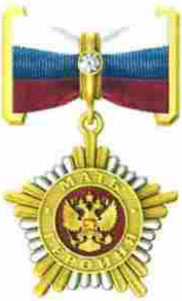
\includegraphics{./figures/medal-front}
		\caption{Лицевая сторона}
	\end{figure}
	\begin{figure}[H]
		\centering
		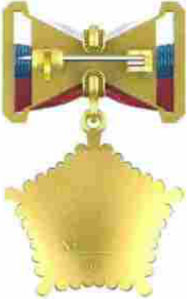
\includegraphics{./figures/medal-back}
		\caption{Оборотная сторона}
	\end{figure}
\eaddition


\baddition{утвержден}{образец}{бланка грамоты о присвоении звания \say{Мать-героиня}}
	\begin{figure}[H]
		\centering
		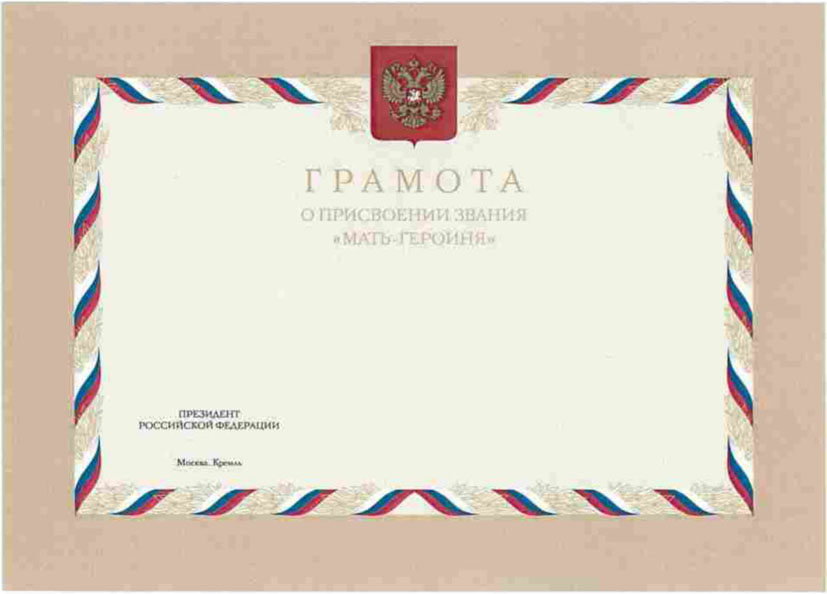
\includegraphics[width=\textwidth]{./figures/charter}
	\end{figure}
\eaddition

\end{document}